% !TeX root = ../main.tex
% Add the above to each chapter to make compiling the PDF easier in some editors.

\chapter{Introduction}\label{chapter:Introduction}


Many public cloud providers emerged in the last decade and gradually commenced to reconstitute the provincial IT infrastructure with their pay as you go pricing model and greater elasticity, these features scaled-down the expenses spent on unutilized resources.
Taking ownership of this reformation, cloud providers and research scientists together brainstormed to deliver consolidated services and transfer the complete provincial IT infrastructure to cloud. \cite{article}
In the mid of last decade the concept of microservices was brought in as a service be the cloud providers, which provided the arena for developers to build, deploy and upgrade complex systems with simple modules.
Though microservices revolutionized in minimizing the complexity of upgrading an complex application by modular upgrade and establishing zero downtime during application upgrade scenarios, microservices imported the complexities associated with distributed system. 
Microservices required many additional resources, which made microservices too complex for smaller application systems and companies.\cite{singleton2016economics}
Recently, public cloud provider popularized the features of serverless computing wherein the developer upload their function code and cloud provider takes the pain deploying, upgrading and monitoring the application.
The automatic management of resources in serverless computing known as Function-as-a-Service (Faas) facilitates application development by offloading resource management to the cloud platform. 
%When extending FaaS to heterogeneous clusters (edge cloud continuum), challenges like communication latencies, function scheduling, and data access patterns grow further.  

When extending FaaS to heterogeneous clusters (edge cloud continuum), where nodes have very limited memory and CPU capacity, are intended to utilize the features like stateless functions and on demand deployment of containerized runtime environment to run their application on cloud by initiating an event of FaaS. \cite{8821843} 
Thus, Serverless Edge computing is incurring challenges like communication latencies, function scheduling, and data access patterns grow further.
Current serverless platforms are limited to clusters of homogeneous nodes and homogeneous functions. 
Although the functions are stateless and thus state changes and look-ups require frequent access to databases, current platforms do not take the data access behavior of functions for scheduling into account. \cite{hellerstein2018serverless}

This thesis focuses on building the performance model of application functions with respect to SLA requirements (response time and latency) for combinations of various resources, such as CPU cores, the network bandwidth, the memory and the number of function replicas and vice versa.
This modelling will facilitate resource management in the continuum and especially function scheduling and data placement.

\newpage

For developing such model, following metrics from three different layers are useful: 

\begin{itemize}
    \item User Centric (SLA)
        \begin{enumerate}
            \item Request Response Time
            \item Number of Requests Served in given time
            \item Latency
        \end{enumerate}
    \item FaaS Platform Centric
        \begin{enumerate}
            \item Number of Function Replicas (which is same as the number of containers)
            \item Number of Invocations (which is same as number of requests served in a given time)
            \item Total Function Response Time (Cold/Warm time + Function Execution time)
        \end{enumerate}
    \item IaaS Centric
        \begin{enumerate}
            \item Number of vCores given to the function
            \item Memory Given to the function
            \item CPU Utilization per time
            \item Memory Utilization per time
            \item Disk I/O per time
            \item Network Bandwidth per time
        \end{enumerate}
\end{itemize}

\section{Problem:}

The number of Internet of Things (IoT) devices are growing exponentially with the development of the Smart City, Connected Car and Industry 4.0. 
As of August 2019, there are 26.6 billion (and growing active) IoT devices in business and consumer space.
The collection of these IoT devices forms a heterogeneous cluster and when these devices triggers millions of events for functions deployed in FaaS, denial of service or increased latency or may be the response to many of these devices.
So, in this Thesis we are building a model which will be capable of responding the user with the required computing, memory and system resources and vice-versa.
This modelling will facilitate resource management in the continuum and especially function scheduling and data placement.

\newpage 

\section{Objective:}

The goal of this thesis is to build these two models for four different types of functions (compute intensive function, memory intensive function, disk I/O intensive function and communication intensive function): 
\begin{enumerate}
\item Given the SLA like response time and Latency, the model will output the
\begin{itemize}
    \item Number of virtual cores required
    \item Memory
    \item Maximum number of function invocations which can be achieved.
    \item Number of function replicas.
\end{itemize}
\item Given the maximum number of cores, memory, and network bandwidth possible, the model will output: 
\begin{itemize}
    \item Avg. request response time
    \item Number of maximum Function invocations
    \item Latency
\end{itemize}
\end{enumerate}
Creation of these models for these types would allow us to create a class of models which can then be used to predict the values for new application functions. 

\section{Test Setup:}

As in the figure 1.1, a kubernetes cluster with 3 nodes (1 master nad 2 workers) are deployed in AWS.
\begin{itemize}
    \item OpenFaaS is deployed on top of kubernetes and the metrics from openfaas are exposed as prometheus metrics.
    \item cAdvisor container is deployed as a pod to extract metrics from kublet and those metrics are also exposed as prometheus metrics.
    \item Kube-state-metrics container is deployed as a pod to extract metrics from pods and those metrics are also exposed as prometheus metrics.
    \item Prometheus is deployed as a pod and configured to read all the exposed metrics from OpenFaaS, cAdvisor and kube-state-metrics and write them to influxdb for long term storage.
    \item InfluxDB is deployed in an separate instance in LRZ cloud services. 
    \item k6 is used as a load testing tool, run from a separate instance and k6 data is pushed to influxdb.
    \item Grafana is also deployed as a pod which helps in visualizing the metrics read by prometheus. Grafana is loaded with three dashboards.
    \begin{itemize}
        \item Kubernetes Pod Metrics (Shows overall cluster CPU / Memory / Filesystem usage as well as individual pod, containers, systemd services statistics. Uses cAdvisor metrics only.)
        \item OpenFaaS Serverless Dashboard (A Dashboard for the OpenFaaS serverless framework)
        \item k6 Load Testing Results (A dashboard for visualizing results from the k6.io load testing tool, using the InfluxDB exporter)
    \end{itemize}
\end{itemize}

\begin{figure}[htpb]
  \centering
  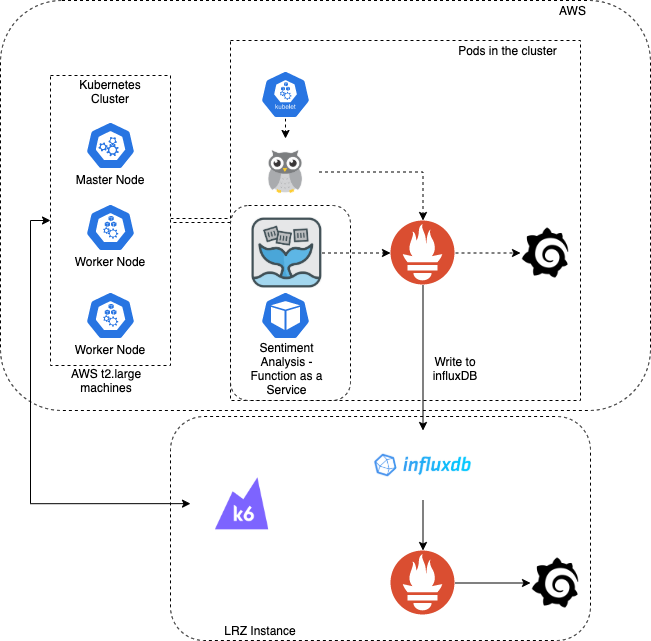
\includegraphics[width=0.8\textwidth]{figures/testSetup}
  \caption{Test Setup} \label{fig:testSetup}
\end{figure}

\newpage 

\section{Approach:}

\subsection{Data Collection:}

\begin{itemize}
    \item Deployed a function on openfaas that can perform sentiment analysis on the text provided. This function is available in openfaas store and can be deployed using the command "faas-cli store deploy sentimentanalysis".
    \item Openfaas prometheus metric exporter exposes metrics like
    \begin{itemize}
        \item Total Invocations
        \item Function Replica Count
        \item Execution duration
        \item Response data
    \end{itemize}

    \item K6 testing tool is used to send data traffic to the function deployed on openfass. Load testing is performed to observe the behavior of the pod's cpu and memory usage.
    \item K6 measurements in influxdb are as follows:
    \begin{itemize}
        \item Number of Virtual Users
        \item Number of Requests per second
        \item Http request duration (response time)
    \end{itemize}

    \item While load testing is done, metrics of the pod's cpu and memory usage are collected by cAdvisor.
    \item cAdvisor prometheus metric exporter exposes metrics like
    \begin{itemize}
        \item Pod CPU usage
        \item Pod memory usage
        \item Pod network I/O
    \end{itemize}
\end{itemize}

\subsubsection{Sample data table:}
\begin{table}[htpb]
  \caption[Data table]{Data Metrics}\label{tab:sample}
    \begin{tabular}{lllllll}
    Time               & CPU Rate              & Mem Utiliz    & HttpReq & res200 & res502 & resTime              \\
    2020-05-17 08:52:10 & 0.12                & 0.00029 & 38.0      & 21.0        & 17.0        & 0.0078         \\
    2020-05-17 08:52:20 & 0.26                & 0.00058 & 92.0     & 43.0        & 49.0        & 0.0077 \\
    2020-05-17 08:52:30 & 0.28                & 0.00058 & 150.0     & 66.0        & 84.0        & 0.0082 \\
    2020-05-17 08:52:40 & 0.29 & 0.00059 & 208.0     & 88.0        & 120.0       & 0.0080 \\
    2020-05-17 08:52:50 & 0.31                & 0.00060 & 273.0     & 110.0       & 163.0       & 0.0077 \\
    2020-05-17 09:03:00 & 1645.40  & 0.96464    & 3600.0     & 787.0       & 2813.0      & 0.8150   \\
    2020-05-17 09:03:10 & 1674.07  & 0.92836    & 3646.0     & 787.0       & 2859.0      & 0.8344   \\
    2020-05-17 09:03:20 & 1706.42  & 0.98191    & 3689.0     & 787.0       & 2902.0      & 0.8551   \\
    2020-05-17 09:03:30 & 1735.42             & 1.01262     & 3737.0     & 787.0       & 2950.0      & 0.8497         \\
    2020-05-17 09:03:40 & 1765.65  & 1.05117     & 3778.0     & 787.0       & 2991.0      & 0.8479   \\
    2020-05-17 09:03:50 & 1795.48             & 1.02082    & 3831.0     & 787.0       & 3044.0      & 0.8678   \\
    2020-05-17 09:04:00 & 1825.44             & 0.99666    & 3885.0     & 787.0       & 3098.0      & 0.8744   \\
    2020-05-17 09:04:10 & 1854.94  & 1.08041    & 3911.0     & 787.0       & 3124.0      & 0.9041  
    \end{tabular}
\end{table}

Considering the above metrics, response time increases with the increase in the number of request per second.

\begin{figure}[htpb]
    \centering
    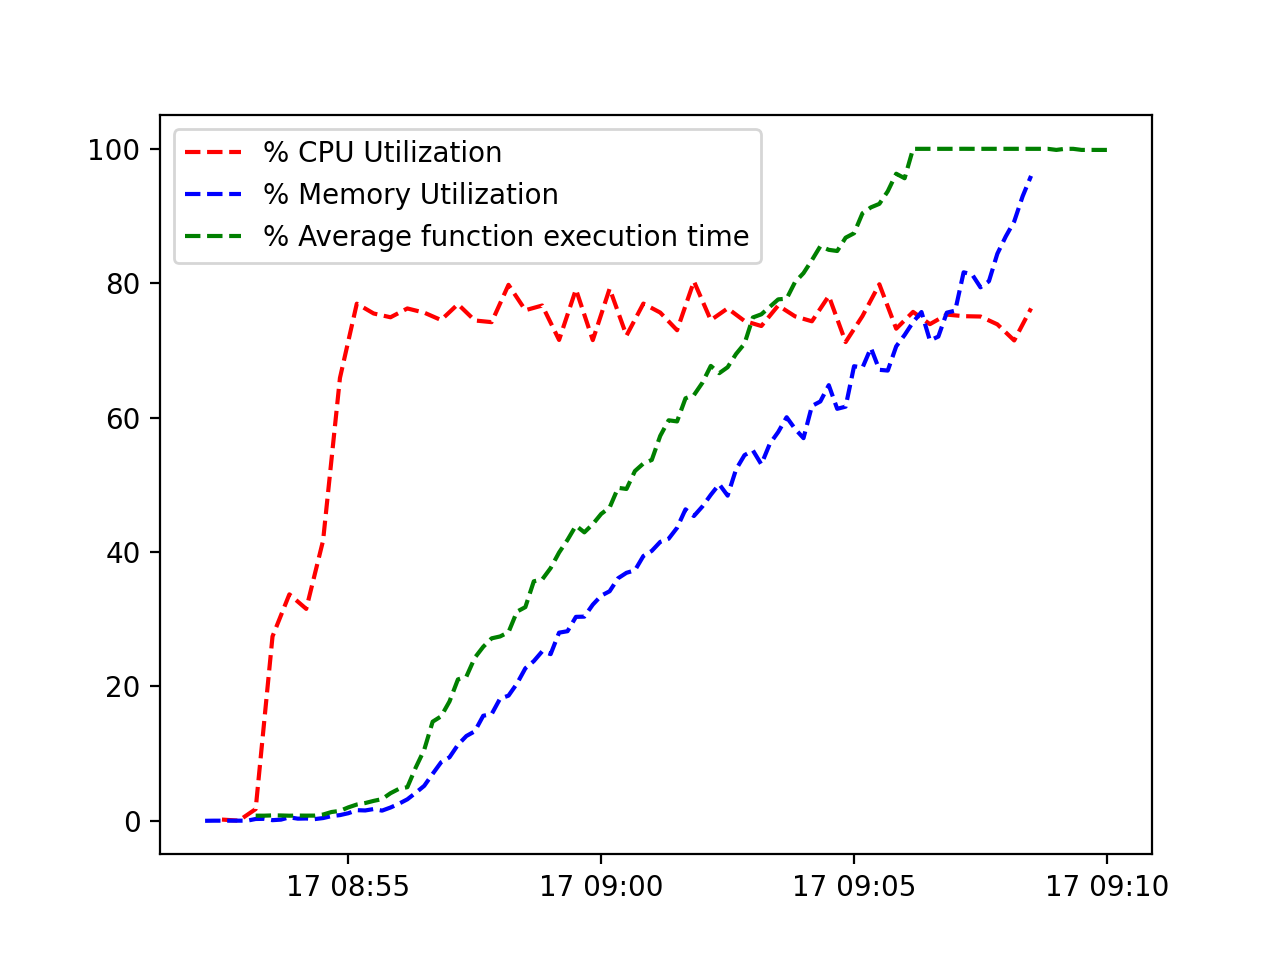
\includegraphics[width=1\textwidth]{figures/cpu_mem_response}
    \caption{Response time increase as the CPU and Memory utilization increases} \label{fig:cpu_mem_response}
\end{figure}

\newpage 

\section{Model Generation:}

By the outcome of the data we hope multiple linear regression would be used as an optimal statistical technique for the current scenario.
As in both of our model, the variables are strongly dependent to one another. 
So on performing a multiple linear regression between Number of virtual cores, memory, function invocations, function replicas, response time and latency would allow us to predict next values of variables based on the current value.

\begin{figure}[htpb]
  \centering
  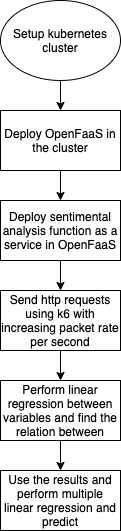
\includegraphics[width=0.2\textwidth]{figures/approach}
  \caption{Overall Approach} \label{fig:approach}
\end{figure}

% The increasing response time for function requests causes a significant drop in the quality of service. 
% The plan of this proposal is to define a stable response time by defining a model which is capable of stating the required resources to acquire a stable response time.
% The figure below states the increase in request per minute increases the cpu rate and memory utilization which inturn defines the constant increase in response time.

% \begin{figure}[htpb]
%   \centering
%   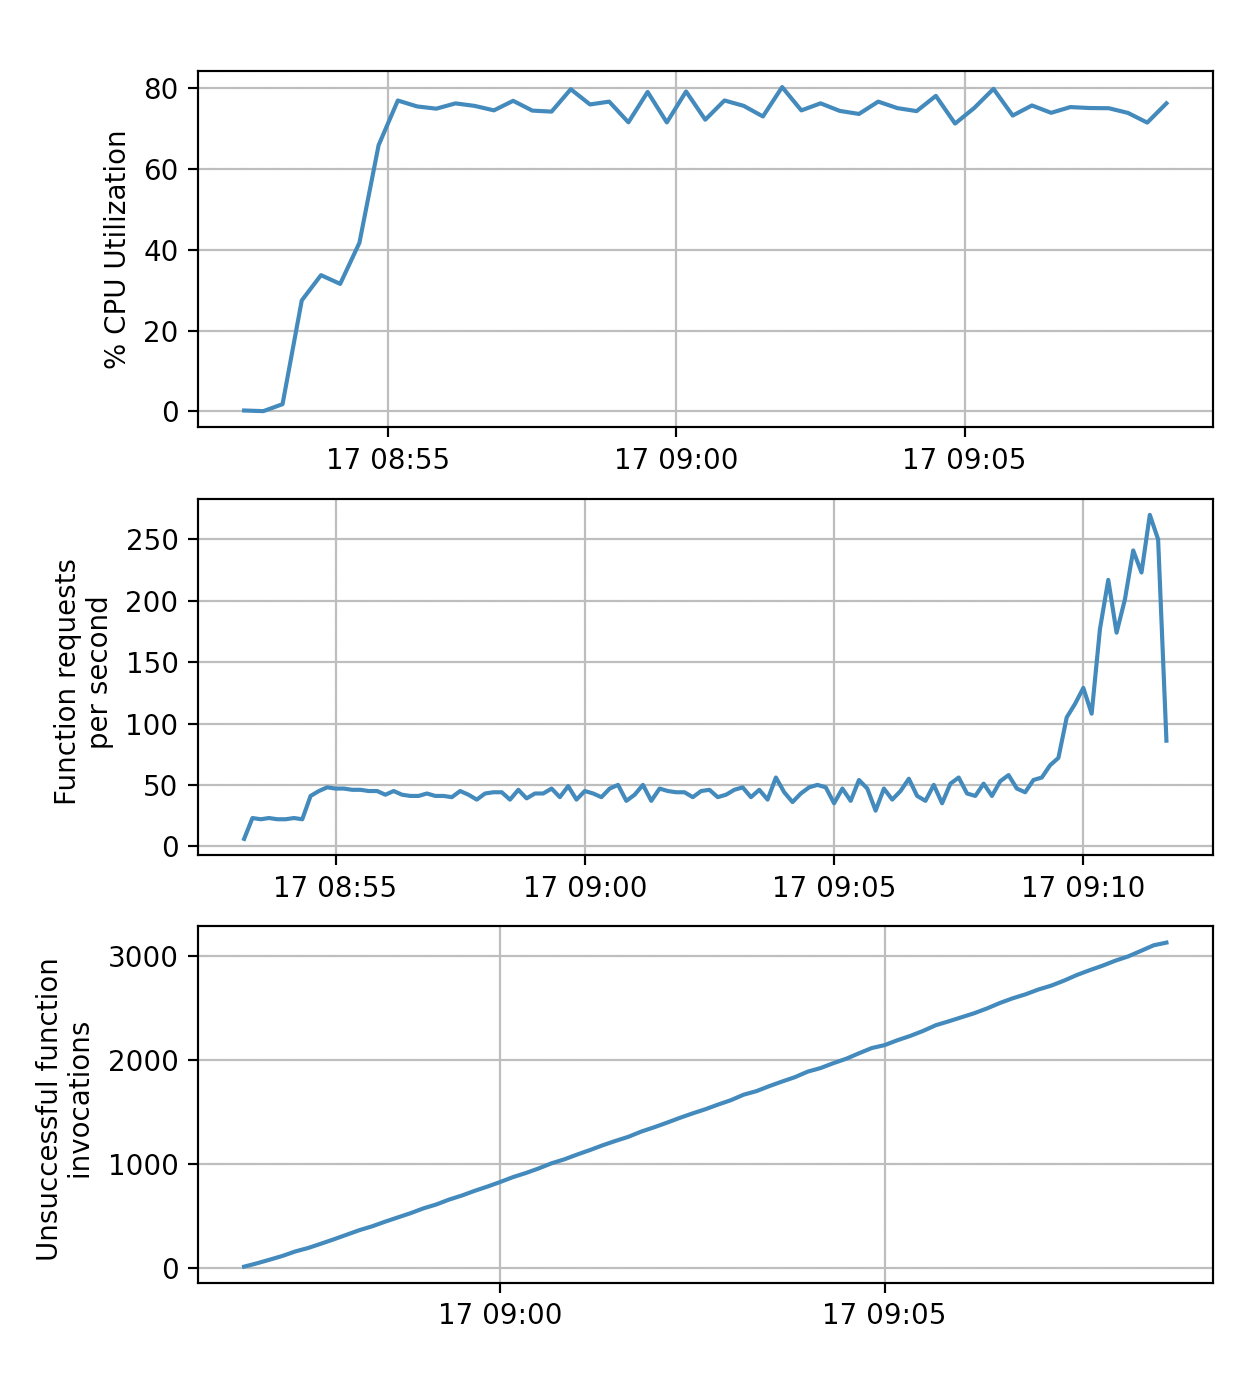
\includegraphics[width=1\textwidth]{figures/graph2}
%   \caption{CPU Rate increases with the increase in number of requests} \label{fig:tumslide}
% \end{figure}

% \begin{figure}[htpb]
%   \centering
%   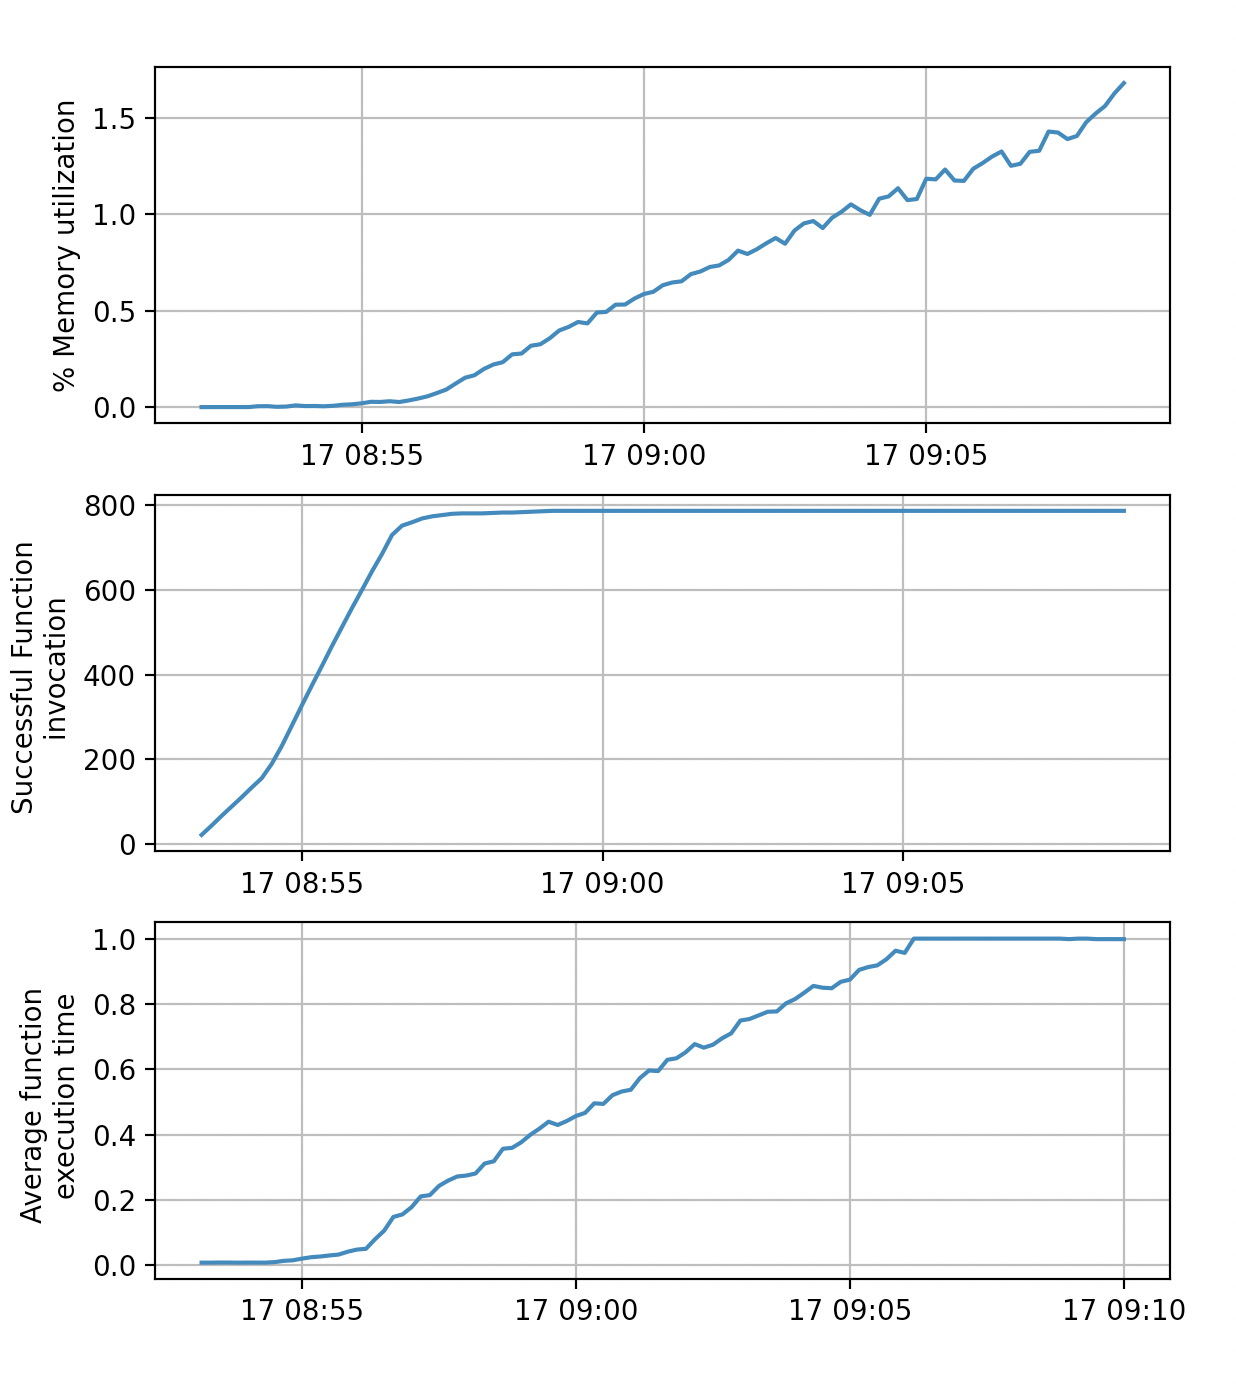
\includegraphics[width=1\textwidth]{figures/graph1}
%   \caption{Response time increases with the increase in memory utilization and CPU rate} \label{fig:tumslide}
% \end{figure}

% \section{Objective:}

% The plan of this proposal is to define a model, that can predict the resources required for a particular response time. 
% Using the metrics below,

% \subsubsection{Types of Metrics:}

% \begin{enumerate}
%     \item User Centric
%     \item FaaS Platform Centric
%     \item IaaS Platform Centric
% \end{enumerate}

% \begin{table}[htpb]
%     \caption[Metrics table]{Types of Metrics}\label{tab:sample}
%     \centering
%     \begin{tabular}{l l l}
%       \toprule
%         User Centric & FaaS Platform Centric & IaaS Platform Centric \\
%       \midrule
%         Cost, & Number of Functions, & Number of Core,\\
%         Response time, & Number of Containers, & Number of Virtual Machines,\\
%         Number of Requests/ & Number of Invocations & Memory used,\\
%         Workload & Execution time (Cold start/ & Storage used \\
%         & Warm start & \\
%         & + Response time) & \\ 
%       \bottomrule
%     \end{tabular}
%   \end{table}

% \section{Outline:}

% \subsubsection{Sample data table:}
% \begin{table}[htpb]
%   \caption[Data table]{Data Metrics}\label{tab:sample}
%     \begin{tabular}{lllllll}
%     Time               & CPU Rate              & Mem Utiliz    & HttpReq & res200 & res502 & resTime              \\
%     2020-05-17 08:52:10 & 0.12                & 0.00029 & 38.0      & 21.0        & 17.0        & 0.0078         \\
%     2020-05-17 08:52:20 & 0.26                & 0.00058 & 92.0     & 43.0        & 49.0        & 0.0077 \\
%     2020-05-17 08:52:30 & 0.28                & 0.00058 & 150.0     & 66.0        & 84.0        & 0.0082 \\
%     2020-05-17 08:52:40 & 0.29 & 0.00059 & 208.0     & 88.0        & 120.0       & 0.0080 \\
%     2020-05-17 08:52:50 & 0.31                & 0.00060 & 273.0     & 110.0       & 163.0       & 0.0077 \\
%     2020-05-17 09:03:00 & 1645.40  & 0.96464    & 3600.0     & 787.0       & 2813.0      & 0.8150   \\
%     2020-05-17 09:03:10 & 1674.07  & 0.92836    & 3646.0     & 787.0       & 2859.0      & 0.8344   \\
%     2020-05-17 09:03:20 & 1706.42  & 0.98191    & 3689.0     & 787.0       & 2902.0      & 0.8551   \\
%     2020-05-17 09:03:30 & 1735.42             & 1.01262     & 3737.0     & 787.0       & 2950.0      & 0.8497         \\
%     2020-05-17 09:03:40 & 1765.65  & 1.05117     & 3778.0     & 787.0       & 2991.0      & 0.8479   \\
%     2020-05-17 09:03:50 & 1795.48             & 1.02082    & 3831.0     & 787.0       & 3044.0      & 0.8678   \\
%     2020-05-17 09:04:00 & 1825.44             & 0.99666    & 3885.0     & 787.0       & 3098.0      & 0.8744   \\
%     2020-05-17 09:04:10 & 1854.94  & 1.08041    & 3911.0     & 787.0       & 3124.0      & 0.9041  
%     \end{tabular}
% \end{table}
